\section{Multivariate Categorization}\label{sec:hmmBdt}

This section describes the separation of the ``pre-cut'' 3-lepton and 4-lepton categories into ``post-cut'' sub-categories in order to enhance the overall sensitivity.
Boosted decision trees (BDTs) are trained using the signal and background simulations in each of these categories.

\subsection{Configuration}
\label{sec:hmmBdtConfiguration}

% Training details
Different classifiers are used for both the 3-lepton and 4-lepton categories, but these share a common setup.
The classifier algorithm used is XGBoost.\cite{xgboost} 

A 5-fold splitting of the available signal and background sample is used.
 Three fifths of each sample define the \emph{training} sample used to fit the BDT.
 One fifth of the sample defines a \emph{validation} sample used to evaluate the performance of the BDT, control the potential for over training to the testing sample, and to select the cuts on the BDT output used for categorization.
 One fifth of the sample defines a \emph{testing} sample which remains blinded until the choices related to the VH channels have been fixed.
 The output of the BDT on the testing sample represent the final result of the BDT and it is essential to refrain from making choices related to the BDT performance on the testing set.
 For example, selecting an optimal cut using the BDT testing set, and then using the same testing set to estimate signal strength, will result in an expected signal amplitude that is larger than that from an unexposed sample 
(e.g. data).
 Making such choices using the \emph{validation} sample avoids this particular complication.

Cross validation is was introduced in order to maximise the benefit from the limited statistics available in simulated events. A cyclic permutation of the 5-fold splitting is used, such that a separate BDT is trained for each fifth of the total sample.

% Samples
Each BDT is trained using the simulated background, with all background components included in the training sample.
The signal for the 4-lepton BDTs are the qqZH samples, while the signal for the 3-lepton BDTs are the W$^\pm$H samples. The per-event weights arising from scale factors and reweighing, along with the event corresponding to the campaign luminosity, cross section, etc are provided to the BDT. Negatively weighted events are removed, and the signal and background weights are both normalized.

% Sample statistics
The available events for training are shown in table \ref{tab:hmmSampleStatistics}.

\begin{table}[htbp]
 \begin{center}
\begin{tabular}{l r r r}\toprule
Sample               & Total Events & Training Events \\
4-lepton signal      & 20700        & 12508    \\
4-lepton background  & 88314        & 53081    \\
3-lepton signal      & 134936       & 80962    \\
3-lepton background  & 185286       & 111107   \\
\bottomrule\end{tabular} 
 \end{center}
 \caption{Numbers of MC events available for training, both in the full sample, and the 3/5 training sample statistics.}
\label{tab:hmmSampleStatistics}
\end{table}

% Training variables
The set of variables provided as input for the BDT was chosen from a larger set of candidate variables.
This set was reduced in order of ascending feature importance (measured by the number of times the variable is used for a decision weighted by the events categorized by the node) until the BDT performance suffers (measured by the AUC).
Different variables are present for the 4-lepton and 3-lepton categories.
The variables for each are listed in Tables \ref{tab:hmm3lepVars} and \ref{tab:hmm4lepVars}.

\begin{table}[htp]
\begin{center}
\begin{tabular}{l l l l}
\toprule
Variable & Definition \\
\midrule
 $\Delta_\phi(E_T^\text{miss},H)$ & $\phi$ between $E_T^\text{miss}$ and the H candidate \\
 $p_T^{l1}$ & W candidate lepton $p_T$ \\
 $m_T(E_T^\text{miss},l1)$ & transverse mass of the W candidate lepton and $E_T^\text{miss}$  \\
 $\Delta_\phi(l1,H)$ & $\Delta$ $\phi$ between H candidate and W candidate lepton \\
 $\Delta_\eta(l1,H)$ & $\Delta$ $\eta$ between H candidate and W candidate lepton \\
 $E_T^\text{miss}$ & missing transverse momentum \\
 $p_T^{j1}$ & $p_T$ of leading jet (if present) \\
 $N_\text{jets}$ & Number of jets \\
\bottomrule
\end{tabular}
\caption{3-lepton variables.}
\label{tab:hmm3lepVars}
\end{center}
\end{table}

\begin{table}[htp]
\begin{center}
\begin{tabular}{l l l l}
\toprule
Variable & Definition \\
\midrule
 $p_T^{j1}$ & $p_T$ of leading jet (if present) \\
 $p_T^{j2}$ & $p_T$ of subleading jet (if present) \\
 $N_\text{jets}$ & Number of jets \\
 $\Delta_\phi(l1,l2)$ & $\Delta$ $\phi$ between the leptons paired for the Z candidate \\
 $\Delta_\phi(Z,H)$ & $\Delta$ $\phi$ between H candidate and Z candidate \\
 $\Delta_\eta(Z,H)$ & $\Delta$ $\eta$ between H candidate and Z candidate \\
 $m_Z$ & Z candidate mass \\
\bottomrule
\end{tabular}
\caption{4-lepton variable.}
\label{tab:hmm4lepVars}
\end{center}
\end{table}

\afterpage{
\begin{figure}[h!]
\captionsetup[subfigure]{position=b}
\centering
\subfloat[][]{{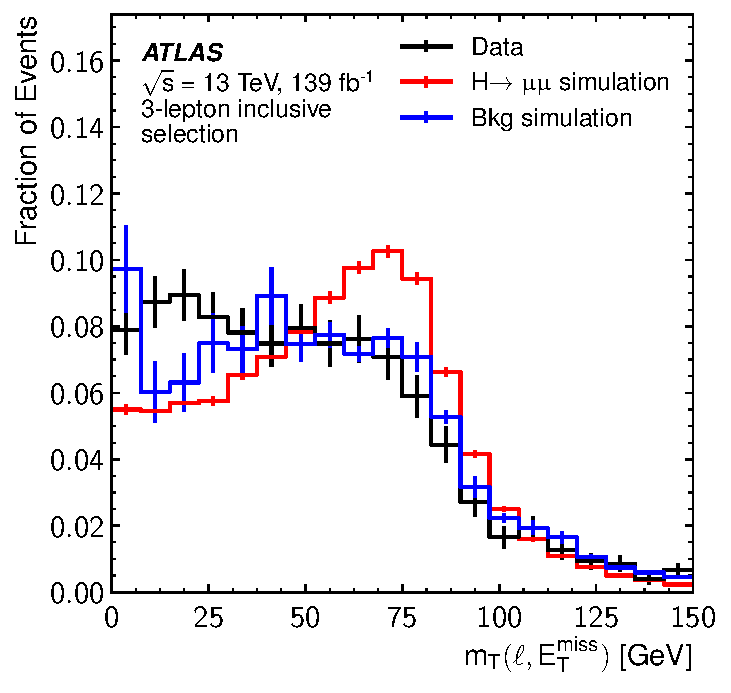
\includegraphics[width=0.35\textwidth]{/home/prime/thesis/draft-text-030820/figures/hmm/public/kine/kine-3lep-aux1_met_mt.pdf}}}
\subfloat[][]{{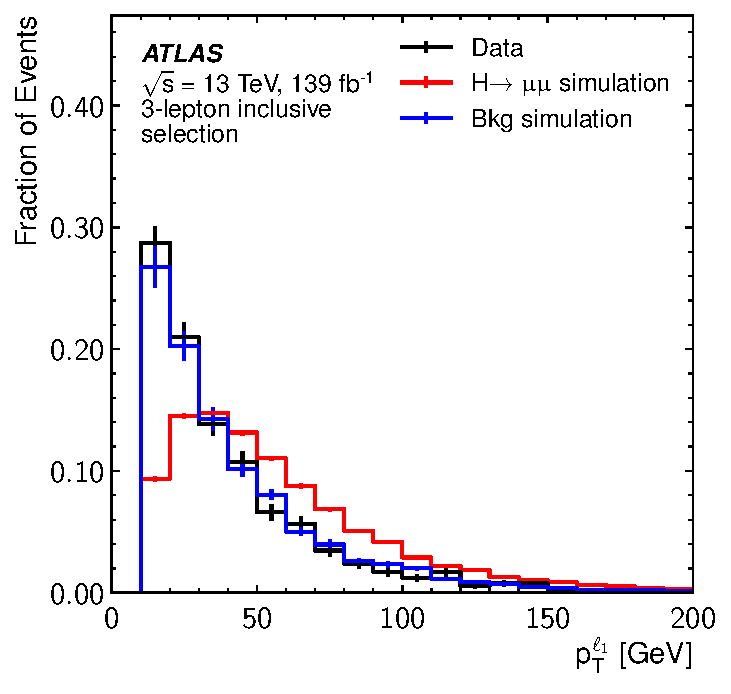
\includegraphics[width=0.35\textwidth]{/home/prime/thesis/draft-text-030820/figures/hmm/public/kine/kine-3lep-aux1_pt.pdf}}}
\subfloat[][]{{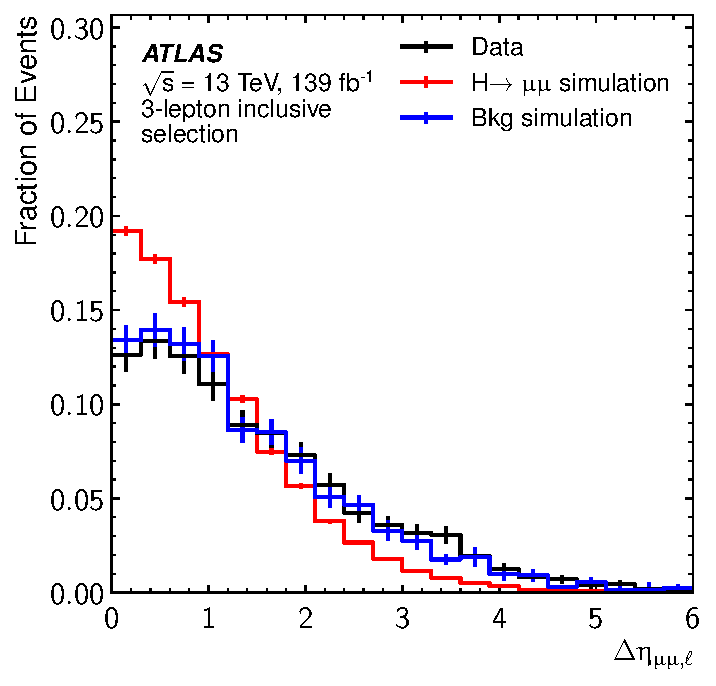
\includegraphics[width=0.35\textwidth]{/home/prime/thesis/draft-text-030820/figures/hmm/public/kine/kine-3lep-aux1_uu_delta_eta.pdf}}} \\
\subfloat[][]{{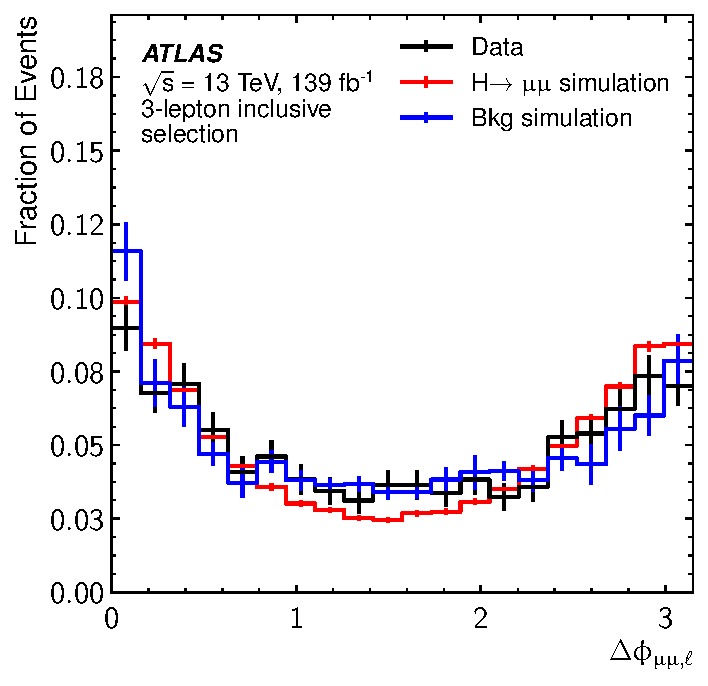
\includegraphics[width=0.35\textwidth]{/home/prime/thesis/draft-text-030820/figures/hmm/public/kine/kine-3lep-aux1_uu_delta_phi.pdf}}}
\subfloat[][]{{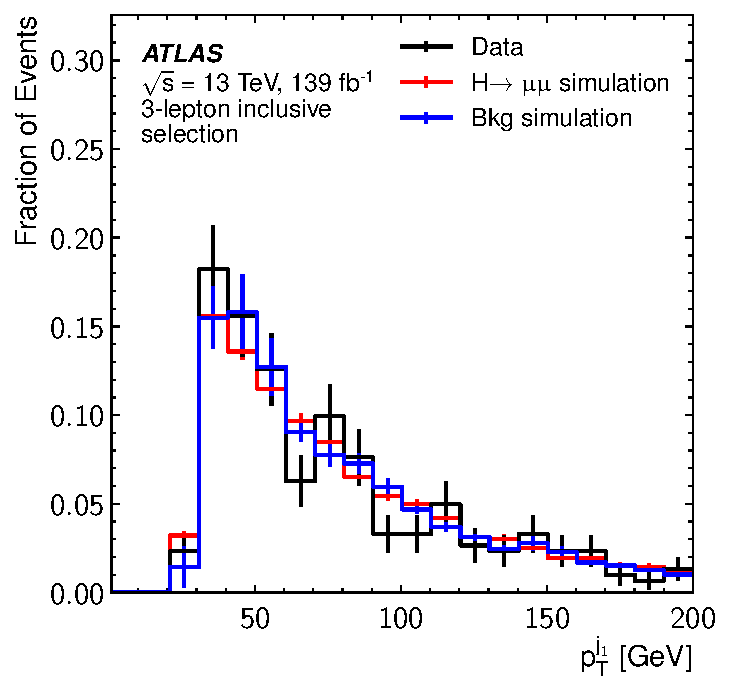
\includegraphics[width=0.35\textwidth]{/home/prime/thesis/draft-text-030820/figures/hmm/public/kine/kine-3lep-j1_pt.pdf}}}
\subfloat[][]{{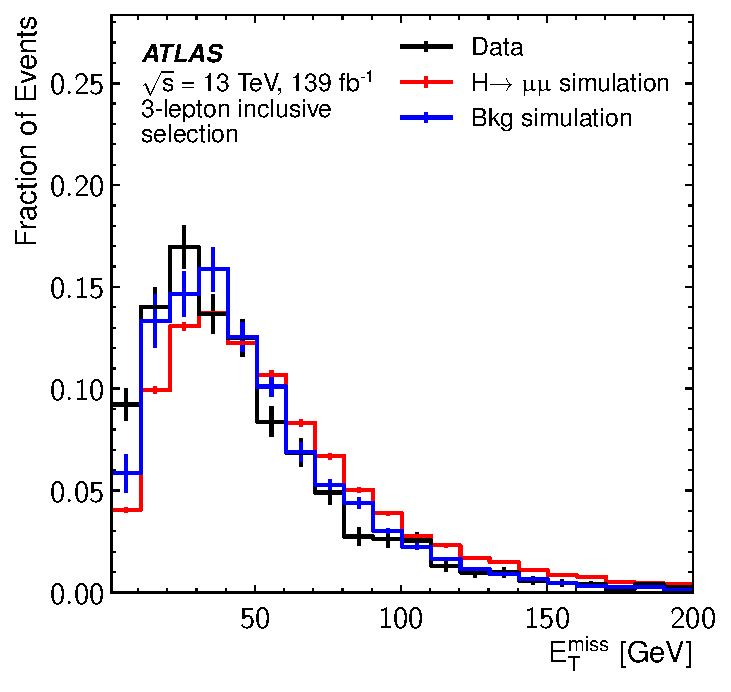
\includegraphics[width=0.35\textwidth]{/home/prime/thesis/draft-text-030820/figures/hmm/public/kine/kine-3lep-met_pt.pdf}}} \\
\subfloat[][]{{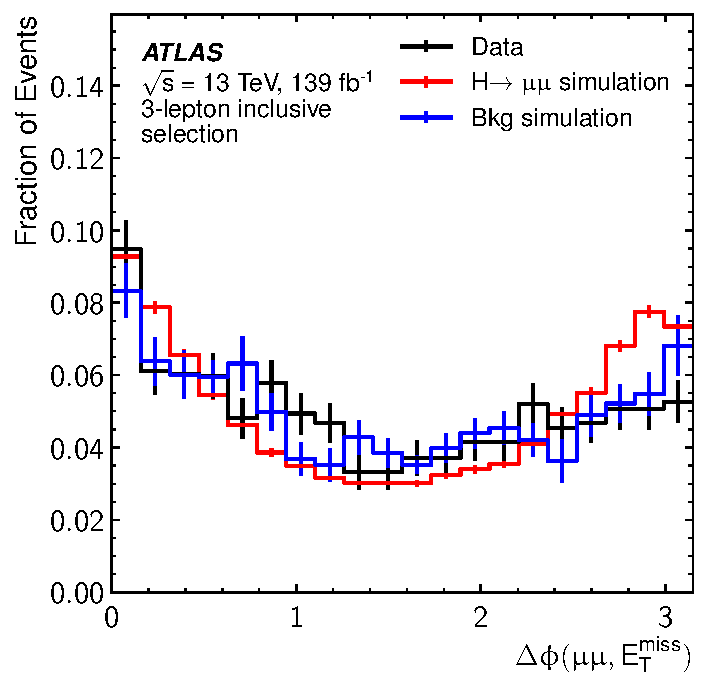
\includegraphics[width=0.35\textwidth]{/home/prime/thesis/draft-text-030820/figures/hmm/public/kine/kine-3lep-met_uu_delta_phi.pdf}}}
\subfloat[][]{{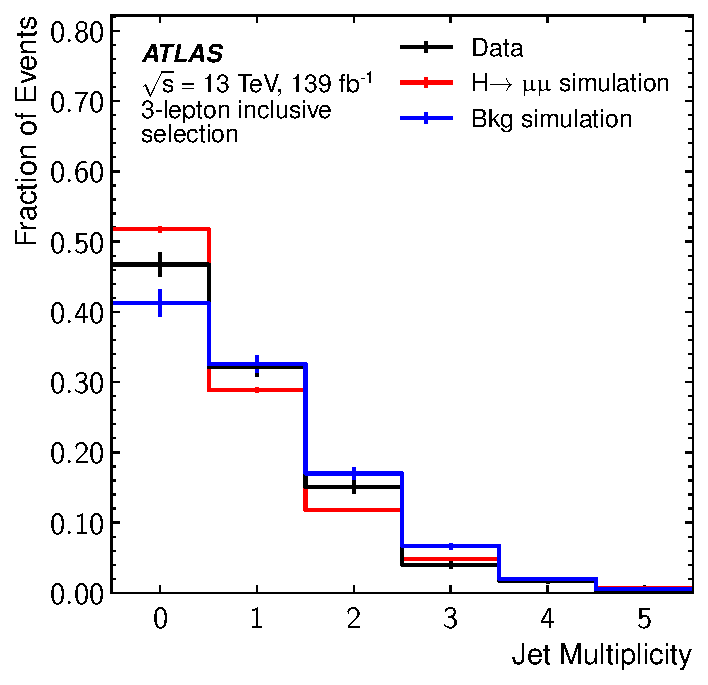
\includegraphics[width=0.35\textwidth]{/home/prime/thesis/draft-text-030820/figures/hmm/public/kine/kine-3lep-nJets.pdf}}}
\caption{Training variables provided as input for the for the 3-lepton classifier. The signal distribution shown in red is comprised of specifically the simulated WH signal dataset, while the background distribution contains all background shown in blue production modes. Data distributions are included in black. Each distribution is normalized, and the error bars on each histogram are statistical only. }
\label{fig:hmm3lepVars}
\end{figure}
\clearpage
}

\afterpage{
\begin{figure}[h!]
\captionsetup[subfigure]{position=b}
\centering
\subfloat[][]{{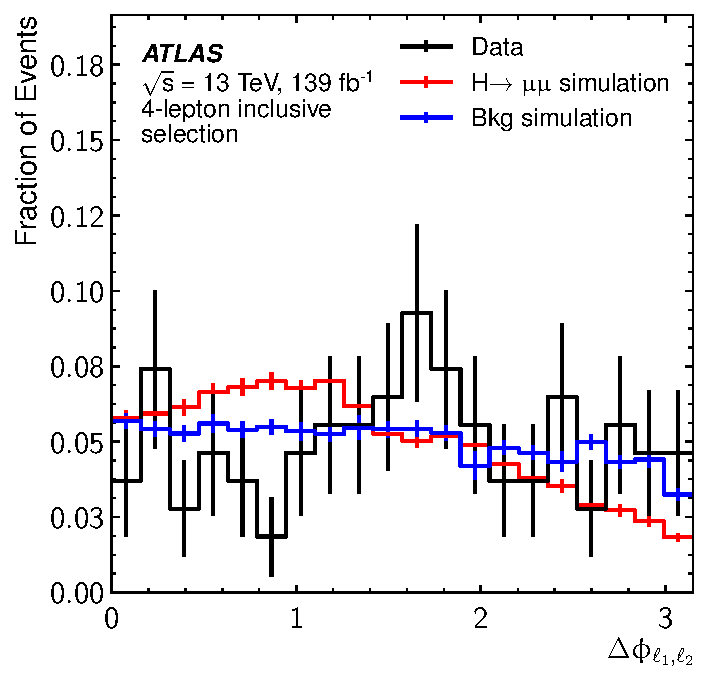
\includegraphics[width=0.35\textwidth]{/home/prime/thesis/draft-text-030820/figures/hmm/public/kine/kine-4lep-auxDilep_delta_phi.pdf}}}
\subfloat[][]{{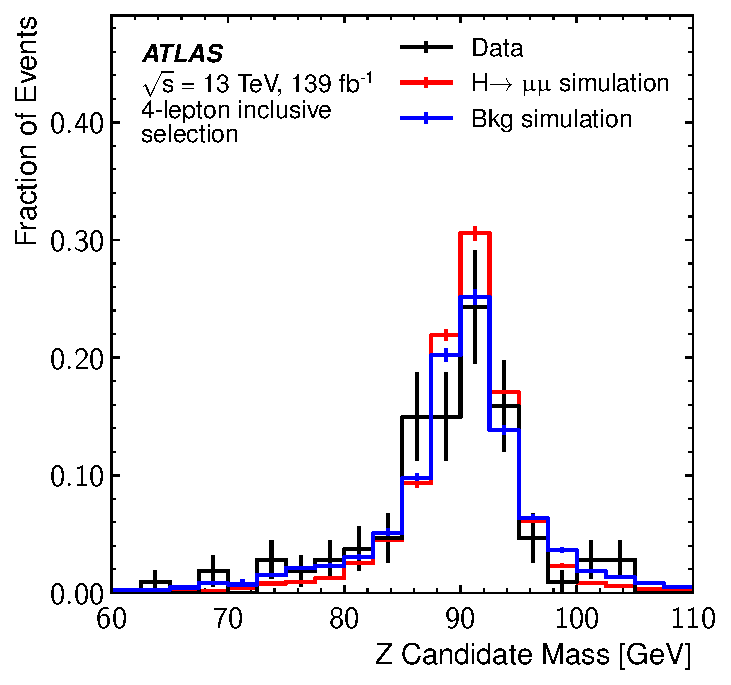
\includegraphics[width=0.35\textwidth]{/home/prime/thesis/draft-text-030820/figures/hmm/public/kine/kine-4lep-auxDilep_mass.pdf}}}
\subfloat[][]{{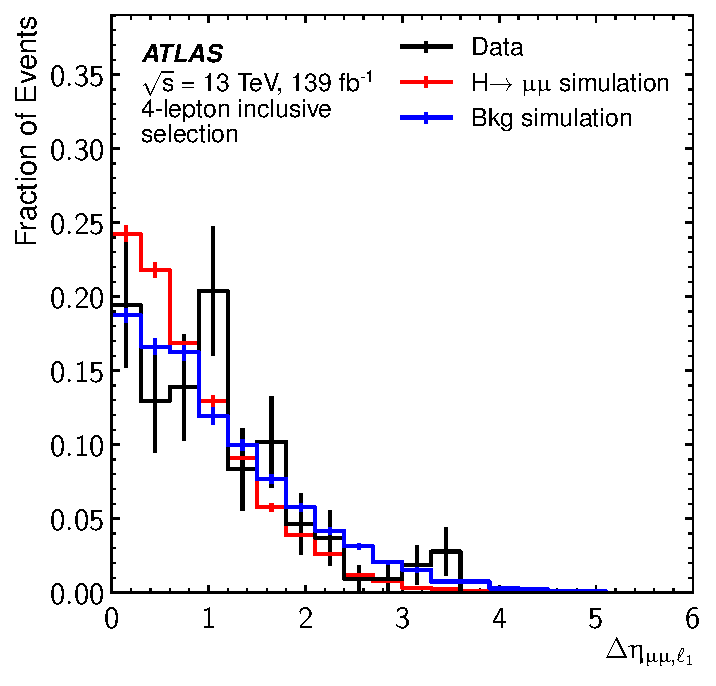
\includegraphics[width=0.35\textwidth]{/home/prime/thesis/draft-text-030820/figures/hmm/public/kine/kine-4lep-aux_uu_delta_eta.pdf}}} \\
\subfloat[][]{{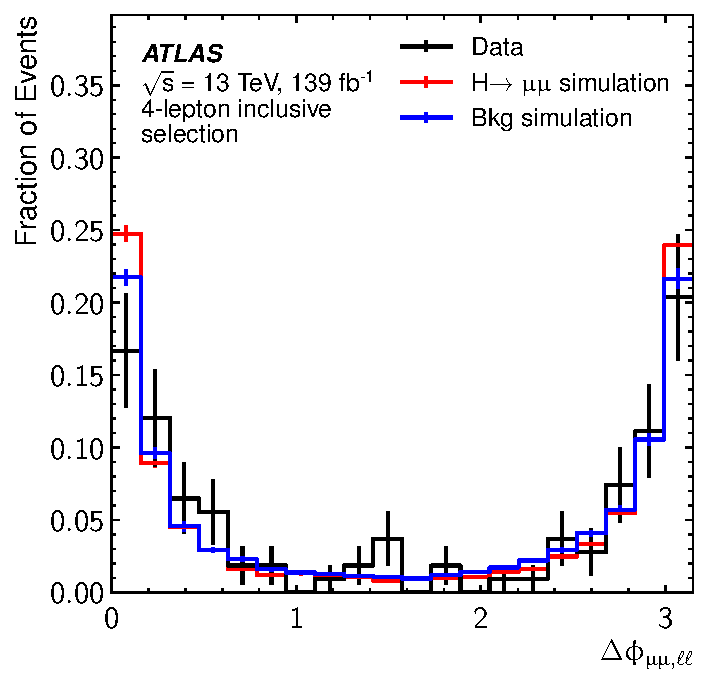
\includegraphics[width=0.35\textwidth]{/home/prime/thesis/draft-text-030820/figures/hmm/public/kine/kine-4lep-aux_uu_delta_phi.pdf}}}
\subfloat[][]{{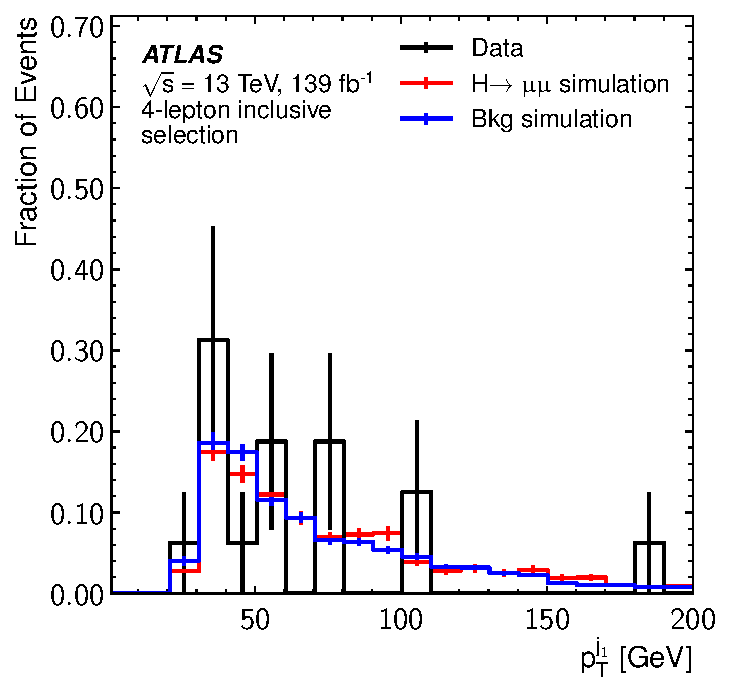
\includegraphics[width=0.35\textwidth]{/home/prime/thesis/draft-text-030820/figures/hmm/public/kine/kine-4lep-j1_pt.pdf}}}
\subfloat[][]{{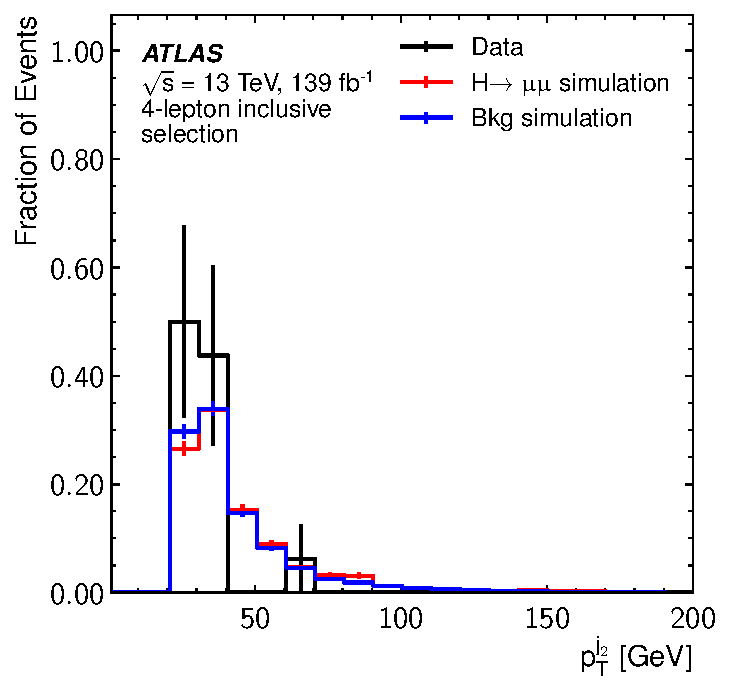
\includegraphics[width=0.35\textwidth]{/home/prime/thesis/draft-text-030820/figures/hmm/public/kine/kine-4lep-j2_pt.pdf}}} \\
\subfloat[][]{{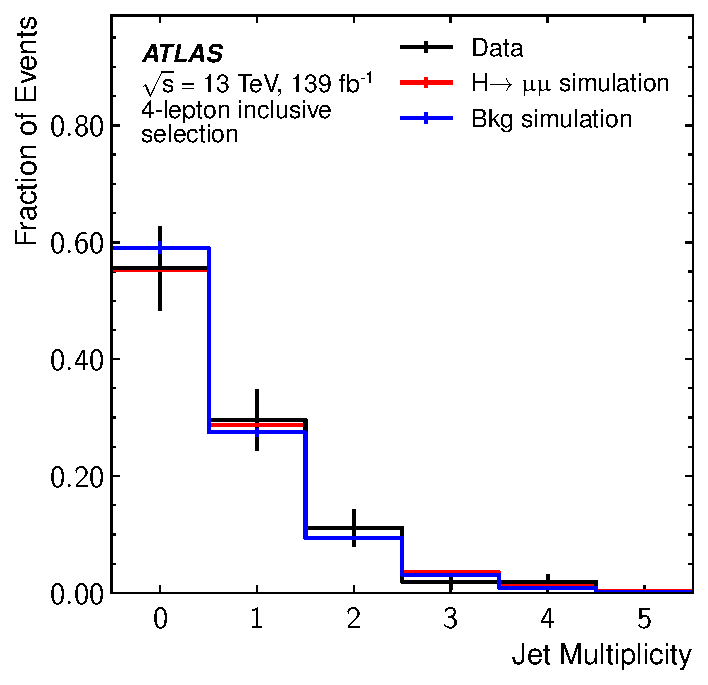
\includegraphics[width=0.35\textwidth]{/home/prime/thesis/draft-text-030820/figures/hmm/public/kine/kine-4lep-nJets.pdf}}}
\caption{Training variables provided as input for the for the 4-lepton classifier. The signal distribution shown in red is comprised of specifically the simulated WH signal dataset, while the background distribution contains all background shown in blue production modes. Data distributions are included in black. Each distribution is normalized, and the error bars on each histogram are statistical only. }
\label{fig:hmm4lepVars}
\end{figure}
\clearpage
}


%%%%%%%%%%%% Variable importance

\begin{figure}[htpb]
  \centering
  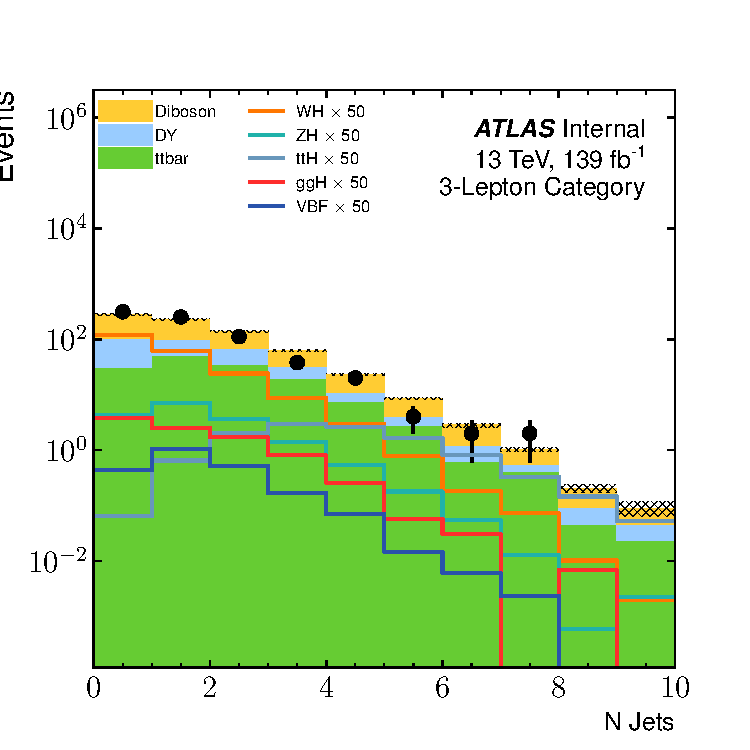
\includegraphics[height=0.48\textwidth]{figures/hmm/nJets/histo-3lep-nJets.pdf}
  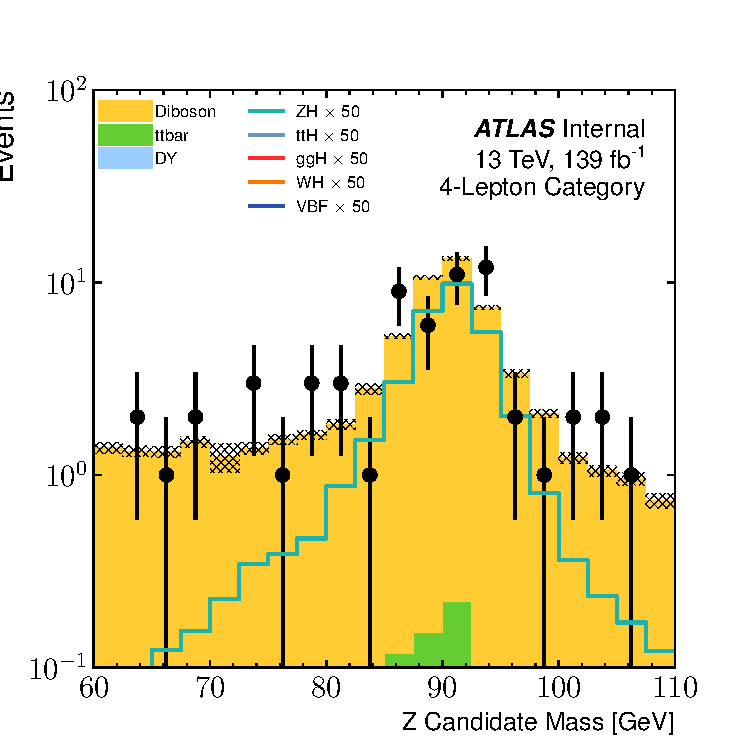
\includegraphics[height=0.48\textwidth]{figures/hmm/zCand/histo-4lep-auxDilep_mass.pdf}
  \caption{Left: N Jets distribution for 3-lepton channel, right: Z candidate mass for 4-lepton channel. These are the highest ranked in feature importance for their category's respective BDT's.}
    \label{fig:hmmImpVars}
\end{figure}

The importance of the variables used in the training are shown in the plots of figure \ref{fig:hmmVarImport}.
In the 4-lepton case, the most important variable is the mass of the Z candidate, which helps identify signal.
In the 3-lepton case the most important variable is the number of jets which helps to separate out Top backgrounds.
The distributions of these two variables are shown in figure \ref{fig:hmmImpVars}.
Detailed definition: \href{https://scikit-learn.org/stable/modules/feature_selection.html}{\underline{here}}.

\begin{figure}[htpb]
  \centering
  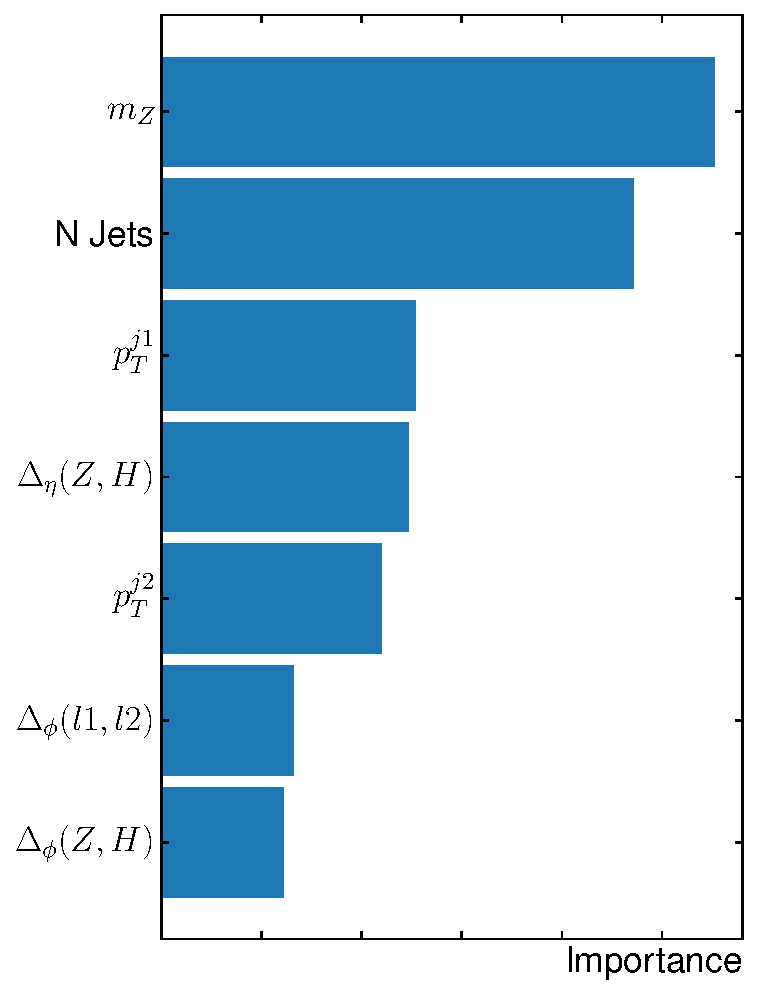
\includegraphics[height=7cm]{figures/hmm/bdtImportance/imp-4lep.pdf}
  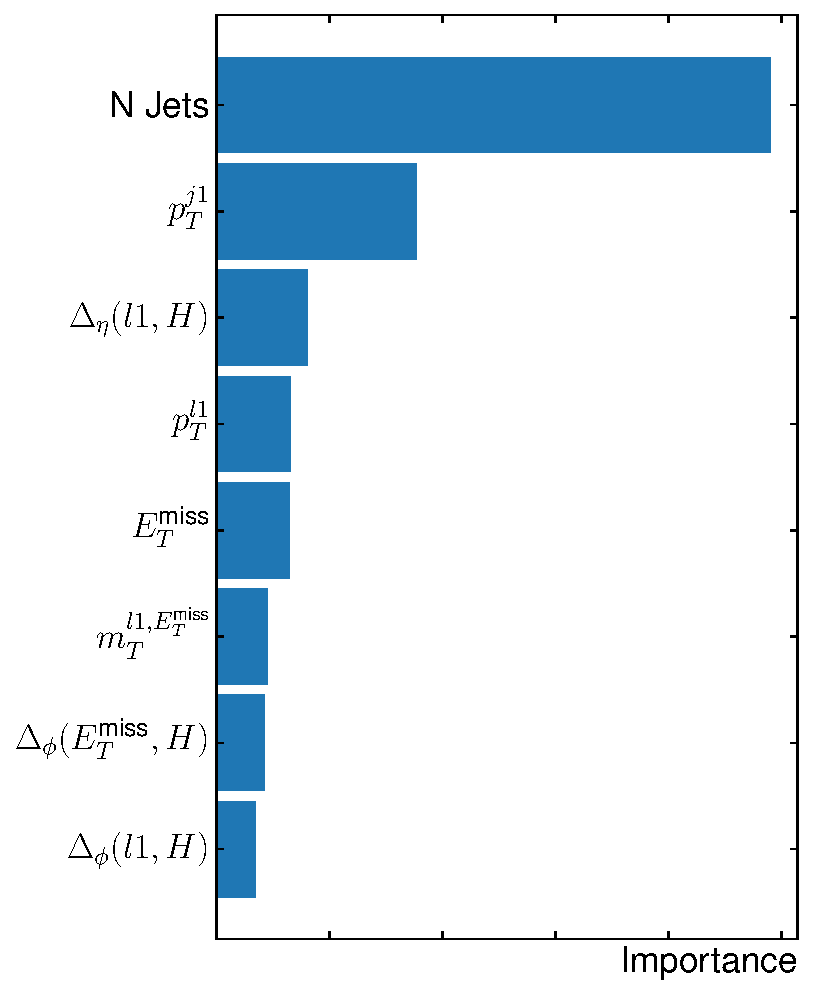
\includegraphics[height=7cm]{figures/hmm/bdtImportance/imp-3lep.pdf}
  \caption{The 4-lepton (left) and 3-lepton (right) variables shown with their respective feature importance, summed over each of the five BDT's trained for each cross validation permutation. $H$ stands for the Higgs candidate, $Z$ for the Z candidate, $l$ for the additional leptons in the event, and $j$ for the jets in the event. The number after the lepton or jet corresponds to the rank of it's $p_T$.}
    \label{fig:hmmVarImport}
\end{figure}

\clearpage

\subsection{Performance}
\label{sec:hmmBdtPerform}

The figure of merit for judging the BDT performance is the area under the receiver operating characteristic (ROC) curve (AUC). The ROC's for representative BDT's are shown for both 3- and 4-lepton categories in figure \ref{fig:hmmBdtRoc}. These show comparable performance for the BDT's of both categories, as well as the impact of the relatively limited statistics of the 4-lepton sample. The signal and background samples shown in the ROC plots correspond to the same samples used for the training, so only WH and ZH signals are shown.

\begin{figure}[htpb]
  \centering
  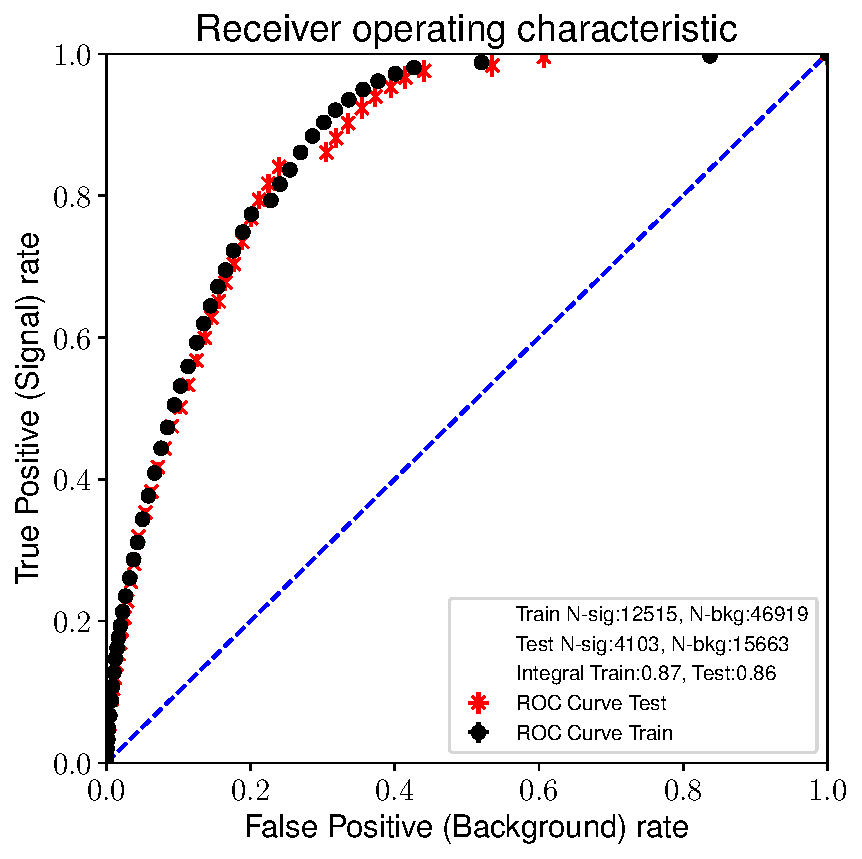
\includegraphics[width=0.48\textwidth]{figures/hmm/bdtHist/roc-4lep-ZH-AllBackground-0-depth2-nEst80tag-new-AllBackground.pdf}
  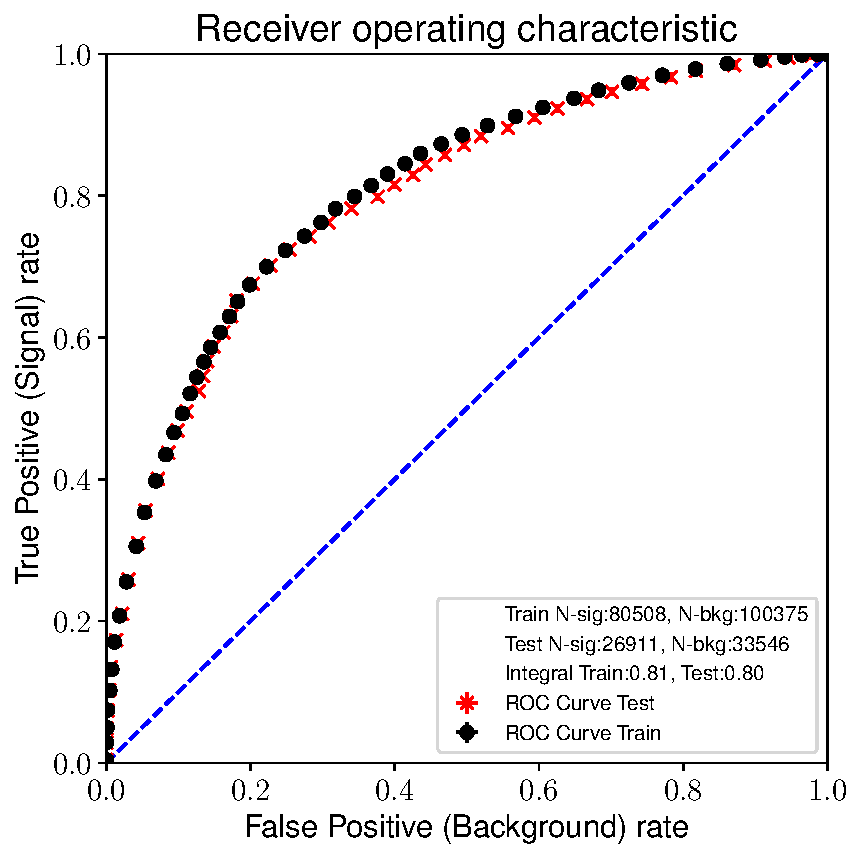
\includegraphics[width=0.48\textwidth]{figures/hmm/bdtHist/roc-3lep-WH-AllBackground-0-depth2-nEst50tag-new-AllBackground.pdf}
  \caption{4 lepton (left) and 3 lepton (right) ROC curves for representative BDT's. Shown in black is the curve for the training set, while red shows the curve for the validation set (labeled test set). Error bars are statistical only. The AUC is labeled on each plot.}
    \label{fig:hmmBdtRoc}
\end{figure}

Figure \ref{fig:hmmBdtScoreLin} shows the BDT discriminant response for different categories of signal and background, scaled the samples cross section and luminosity. The signal/background separation is more apparent in this plot than in those normalized to the physical expectation.


\begin{figure}[htpb]
  \centering
  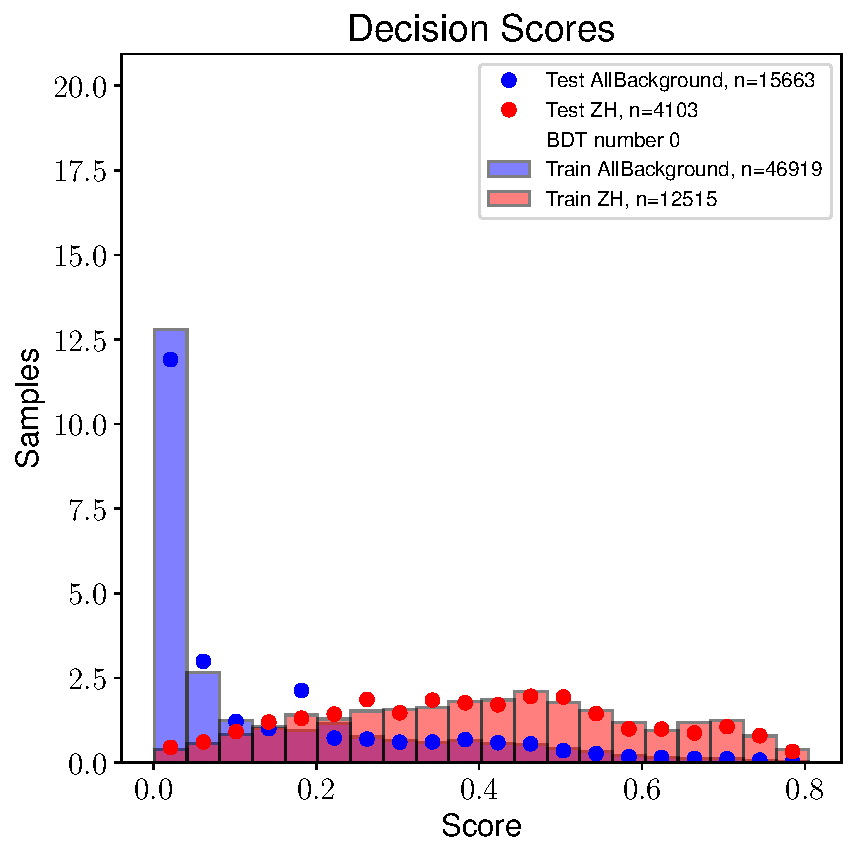
\includegraphics[width=0.48\textwidth]{figures/hmm/bdtHist/bar20-4lep-ZH-AllBackground-0-depth2-nEst80tag-new-AllBackground.pdf}
  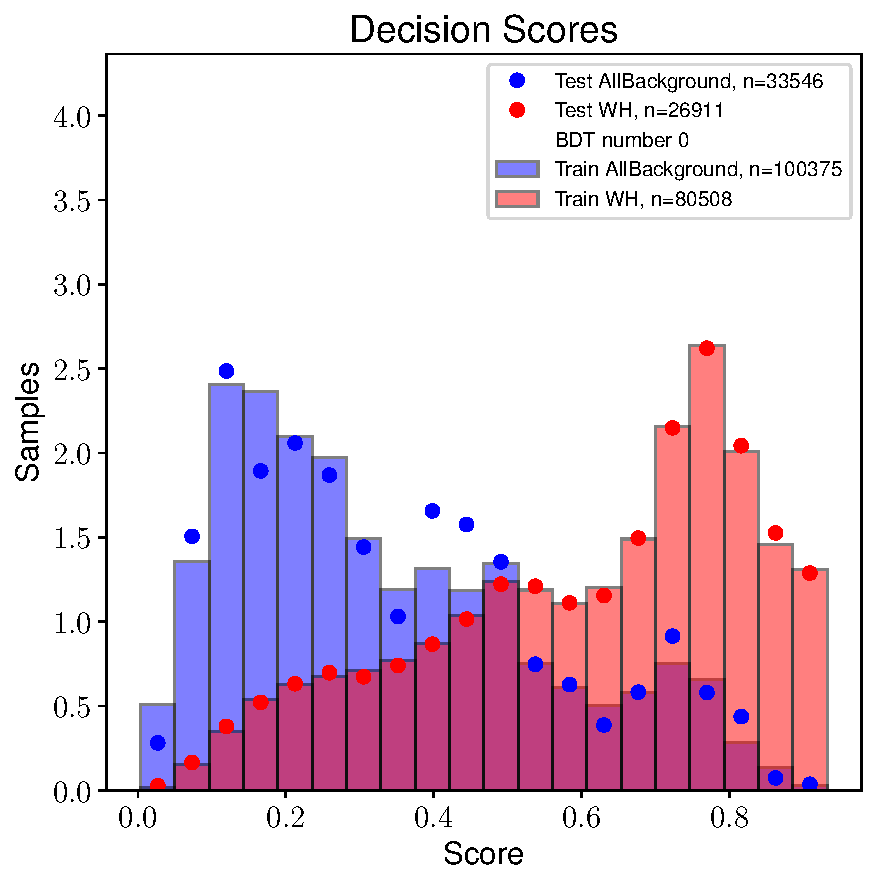
\includegraphics[width=0.48\textwidth]{figures/hmm/bdtHist/bar20-3lep-WH-AllBackground-0-depth2-nEst50tag-new-AllBackground.pdf}
  \caption{4 lepton (left) and 3 lepton (right) distributions of the BDT discriminant, where the signal and background samples share a normalization. The signal distribution is that of the sample used for training, not the full signal MC sample.}
    \label{fig:hmmBdtScoreLin}
\end{figure}

Figure \ref{fig:hmmBdtScore} shows the BDT discriminant response for different categories of signal and background, scaled the samples cross section and luminosity. The composition of the background and signal is more apparent in these plots: primarily the target signal production mechanism is separated. Top backgrounds are particularly well separated owing in part to the high statistics available for these samples.

For 4-lepton case, category ``VH4Lep-High'' is selected by requiring 4-lepton BDT 
score greater than 0.12. 
And for 3-lepton case, two categories ``VH3Lep-High'' and ``VH3Lep-Low'' are selected. The former
is selected by requiring 3-lepton BDT score greater than 0.7,
and the latter is selected by requiring 3-lepton BDT score less than 0.7
but greater than 0.1.
The events failing VH categorization selection are sorted into ggF and
VBF categories as described in Section \ref{sec:hmmCategorization-ggF-VBF}.
 
\begin{figure}[htpb]
  \centering
  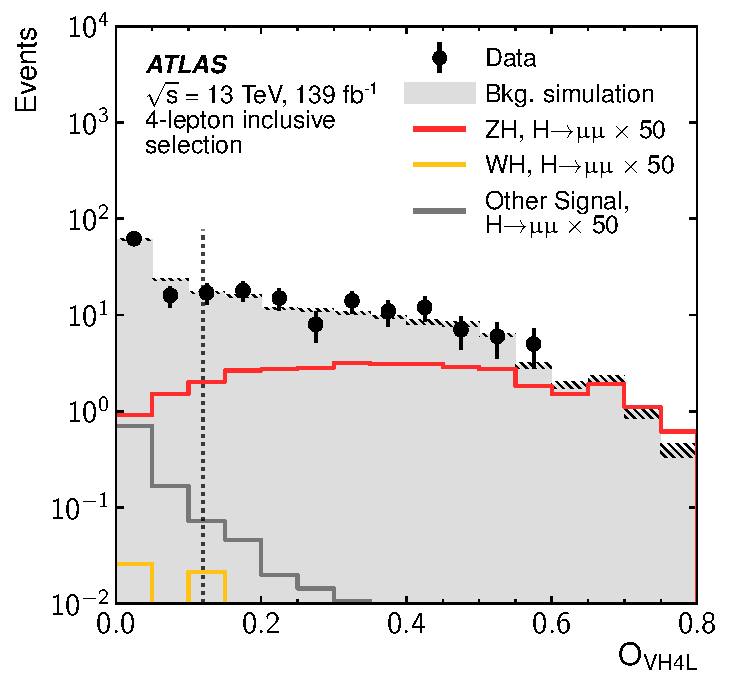
\includegraphics[width=0.48\textwidth]{figures/hmm/public/bdt/histo-4lep-bdtScore.pdf}
  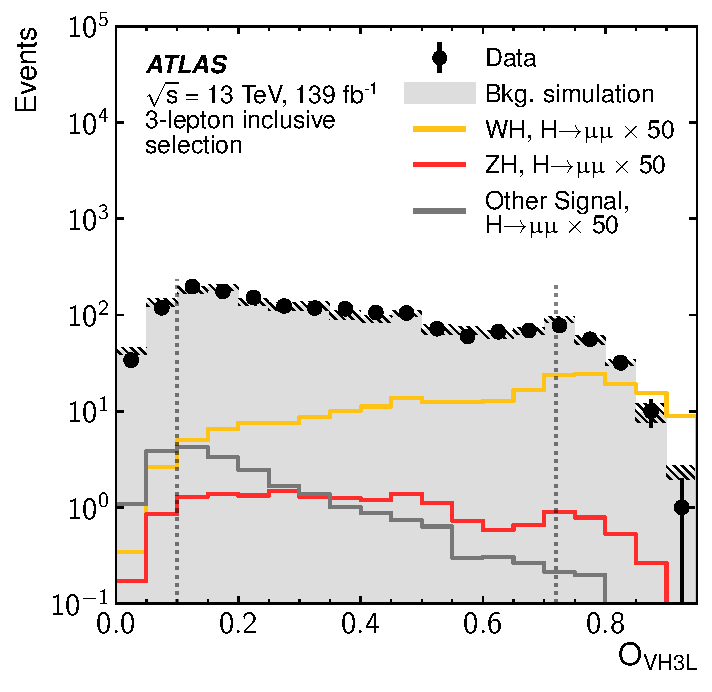
\includegraphics[width=0.48\textwidth]{figures/hmm/public/bdt/histo-3lep-bdtScore.pdf}
  \caption{4-lepton (left) and 3-lepton (right) distributions of the BDT discriminant, using the final test scores. The simulated background is shown in shaded grey, while the signal distributions are drawn as lines in red for ZH and orange for WH. The remaining non-VH production mechanisms (ggF, VBF, and ttH) are combined and plotted as a dark grey line. All the signal histograms have been scaled by a factor of 50 to enhance visibility.\\
  It is clearly observed that the score separates signal to the left and background to the right. Of similar importance is that it specifically isolates the VH signal of interest, and not the other signal productions. For 4-lepton this is the ZH signal and for 3-lepton this is the WH signal. Vertical dotted lines indicate the values that delineate which events belong in which final categories. The full dataset is included as well, which is used to fix the normalization of the background. \\
  Comparing the separation power of the two discriminant, the 3-lepton discriminant is more powerful. This is due in part to the stricter 4-lepton event selection, which is able to remove many more ``easily'' separable background events. The remaining events are more similar topologically to the ZH signal.}
    \label{fig:hmmBdtScore}
\end{figure}

\subsection{Categorization}

The event selection results in two selections: 4-lepton and 3-lepton.
Next, using the BDT discriminant scores, these selections are further divided into sub-categories based on the relative purity of the signal.
The 4-lepton category is divided once into low-purity and high-purity categories.
The 3-lepton category, since the event multiplicity is higher, is divided into low-, medium-, and high-purity categories.

Each event belongs to both a validation dataset and a testing dataset, each of which has an associated discriminant score.
The validation scores are considered when selecting the score thresholds between categories.
The testing scores are used for the final hypothesis test and limit setting.
An optimization scan over various thresholds of the expected significance is performed.
The choice of thresholds made that results in the highest expected significance using the validation scores.
These are specified in Table \ref{tab:hmmBdtCuts}.

\begin{table}[htp]
\begin{center}
\begin{tabular}{l l l l}
\toprule
Category & Discriminant \\
\midrule
4-Lepton High-purity & $O\ge0.12$ \\
4-Lepton Low-purity & $O<0.12$ \\
3-Lepton High-purity & $O\ge0.72$ \\
3-Lepton Middle-purity & $0.10\ge O<0.72$ \\
3-Lepton Low-purity & $O<0.10$ \\
\bottomrule
\end{tabular}
\caption{Category definitions based on the ranges of the discriminant value $O$. The output of the BDT is scaled such that $O\in[0,1]$.}
\label{tab:hmmBdtCuts}
\end{center}
\end{table}

To pick the score thresholds using the testing set, and then perform a hypothesis test in categories defined by that threshold, would lead to a misleading signal and background expectation in those categories.
The choice of threshold would be biased to the statistical fluctuations in the test dataset.
This results in categories biased to contain more simulated signal events and fewer simulated background events than would be expected in the data.
Since analysis on the data includes the signal model based on simulation, such a method is unacceptable.

\begin{figure}[htpb]
  \centering
  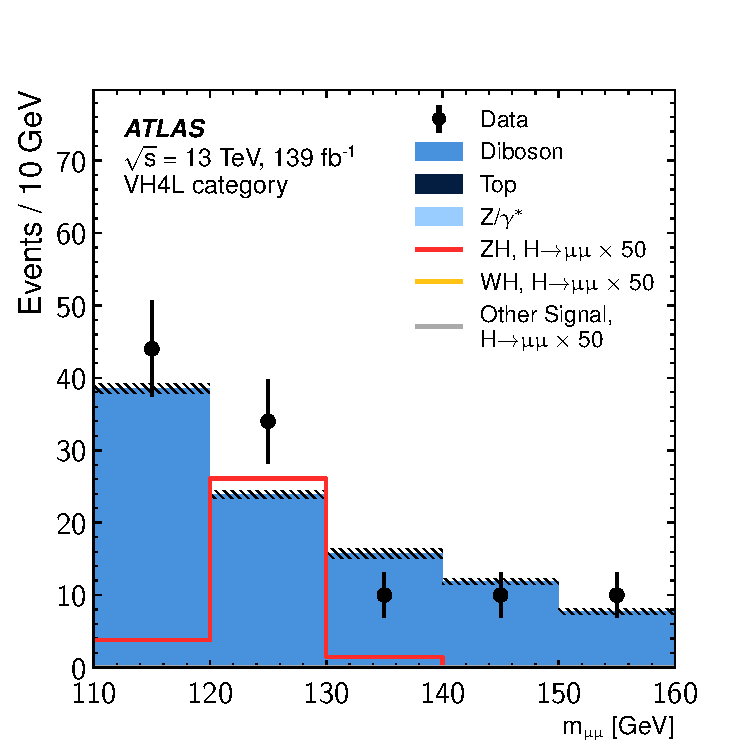
\includegraphics[width=0.45\textwidth]{figures/hmm/public/postCut/histo-4lep0-muu.pdf} \\
  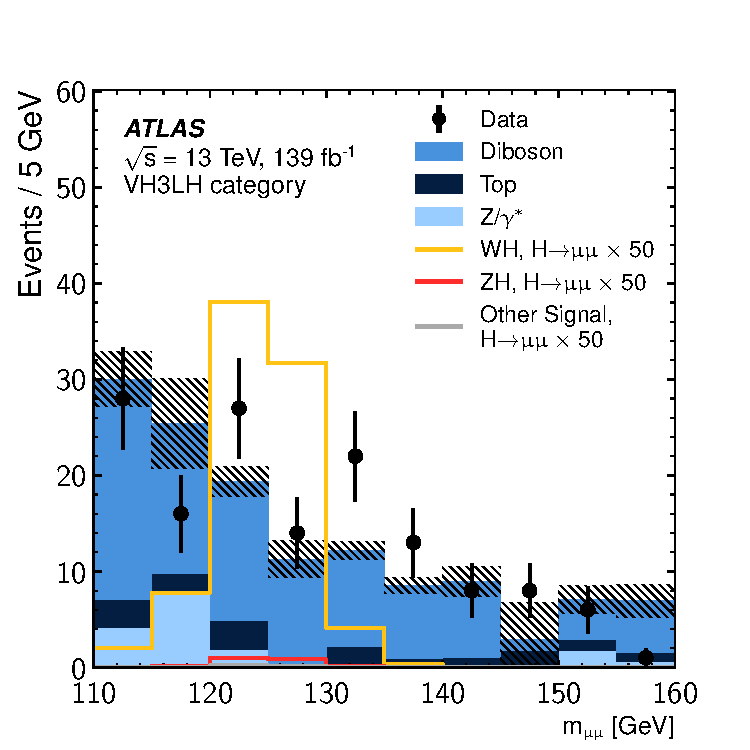
\includegraphics[width=0.45\textwidth]{figures/hmm/public/postCut/histo-3lep0-muu.pdf} 
  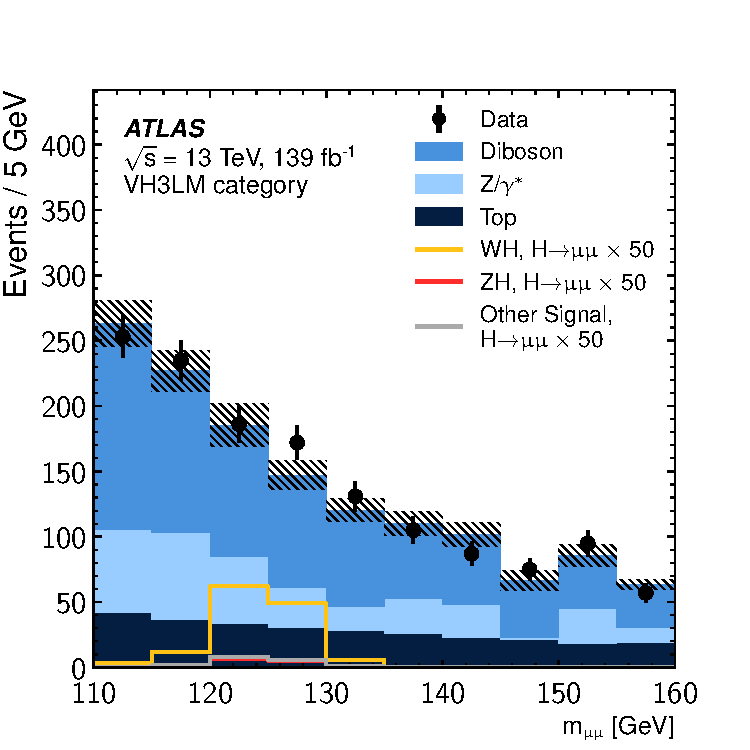
\includegraphics[width=0.45\textwidth]{figures/hmm/public/postCut/histo-3lep1-muu.pdf} 
  \caption{Distributions of \muu in the 4-lepton (top) and 3-lepton (bottom) categories after a cut on the BDT discriminant.}
    \label{fig:hmmPostcutMassHists}
\end{figure}
\clearpage

The high and middle-purity categories are considered for further analysis, while the low-purity events are only analyzed in the inclusive categories defined before the BDT cut.
The distributions of \muu are shown in Figures \ref{fig:hmmPrecutMassHists} and \ref{fig:hmmPostcutMassHists}.
The former shows the inclusive distribution before further categorization with the BDT discriminant.
The latter shows the distributions in the categories defined in Table \ref{tab:hmmBdtCuts}.
The motivation to use the discriminant becomes apparent in these plots when compared to Figure \ref{fig:hmmPrecutMassHists}.
In both the 4-lepton and 3-lepton high-purity categories, Drell-Yan production has been essentially removed.
The background remaining is primarily from diboson sources.
The purity of the signal selection is also clear in the high-purity categories: the categories select for homogeneous ZH or WH depending on their target.

